%Note di Ingegneria del Software
%Sommario: Diagrammi delle classi, Tipi di dipendenze

\cornell{Diagrammi delle classi}{Descrivono il \textbf{tipo di oggetti} che fanno parte del sistema\\
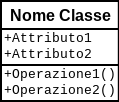
\includegraphics[scale=0.5]{images/21.png}\\
L'unica parte obbligatoria è il nome della classe. Il resto sono dette "features".\\
Il blocco completo è detto, ovviamente, classe}
\cornell[Nota]{Classe vs Oggetto}{La classe è una "blueprint", che definisce come istanziare gli oggetti.\\
L'oggetto è \textbf{l'istanziazione} della classe}
\cornell{Attributi}{Si definiscono in una sezione della classe, con la seguente sintassi:\\
\texttt{visibilità nome: tipo [molteplicità] = default \{proprietà aggiuntive\}}\\
Dove visibilità può essere \begin{description}
\item [+] Pubblica
\item [-] Privata
\item [\#] Protetta
\item [\textasciitilde] Di Package
\end{description}\\
Un esempio può essere: \texttt{\#pippo: string}}
\cornell{Relazioni Fra Classi (Associazioni)}{ 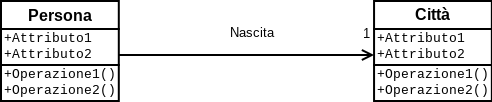
\includegraphics[scale=0.5]{images/22.png}\\
È una notazione alternativa e meno invadente di\\
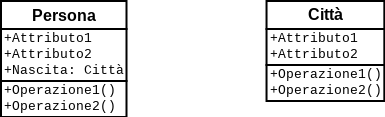
\includegraphics[scale=0.5]{images/23.png}\\
solitamente quest'ultima è usata se B è un tipo primitivo, oppure se il diagramma è già molto confuso.\\
Anche se è possibile inserire la visibilità dell'associazione vicino al nome, questa viene solitamente definita private (in mancanza di simboli)}
\cornell{Molteplicità}{ \begin{itemize}
\item 1 (Sicuramente è presente una istanza)
\item 0..1 (Nessuna o una sola istanza)
\item * oppure 0..* (qualunque numero di istanze)
\item 1..*
\item \text{[2,5]} (da due a 5 istanze)
\end{itemize}}
\cornell{Proprietà aggiuntive}{Solitamente le proprietà aggiuntive più usate sono \begin{itemize}
\item Ordered (Per i vettori o gli array ad esempio)
\item Unordered (Per i set)
\end{itemize}}
\cornell{Associazioni}{Anche se le associazioni è etichettata con un verbo, bisogna usare nomi.\\
Evitare associazioni bidirezionali (che sarebbero delle dipendenze circolari.)}
\cornell{Esempio}{ 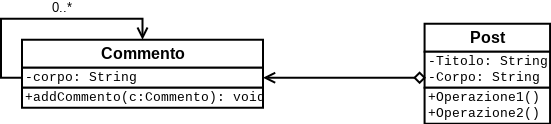
\includegraphics[scale=0.5]{images/24.png}}
\cornell{Operazioni}{Si scrivono sempre nel diagramma delle classi con la seguente sintassi:\\
\texttt{visibilità nome (lista parametri): ritorno {proprietà}}\\
Dove ogni membro della lista parametri ha la seguente sintassi:\\
\texttt{direzione nome:tipo=default}\\
Direzione può essere: \begin{itemize}
\item in: Valore non modificato dal metodo (default)
\item out: Valore che può essere modificato dal metodo, da evitare
\item inout
\end{itemize}\\
Un esempio può essere:\\
\texttt{+addCommento(in c:Commento): void}}
\cornell[Cavilli tecnici]{Operazione Vs Metodo}{Operazione e Metodo non sono la stessa cosa:\\
L'operazione è la "firma del metodo", quindi indipendente dall'implementazione singola.\\
Il metodo è l'implementazione/corpo dell'operazione.}
\cornell{Commenti E Note}{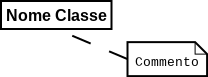
\includegraphics[scale=0.5]{images/25.png}\\
I commenti possono essere legati alla classe, ad un attributo o ad una operazione. Il loro scopo è aggiungere informazioni utili al diagramma.}
\cornell{Dipendenza}{Si ha dipendenza tra due elementi se la modifica della definizione del primo può cambiare la definizione del secondo.\\
È simboleggiata da una freccia con linea tratteggiata\\
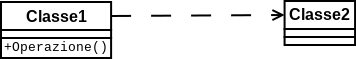
\includegraphics[scale=0.5]{images/26.png}\\
Le dipendenze vanno \textbf{minimizzate} (Loose Coupling).\\
Più codice condiviso c'è tra due tipi e maggiore è la dipendenza tra le classi.}
\cornell{Tipi di Dipendenze}{ \begin{itemize}
\item $\langle\langle$ call $\rangle\rangle$ - Invocazione di un'operazione nella classe di destinazione
\item $\langle\langle$ create $\rangle\rangle$ - Creazione di istanze
\item $\langle\langle$ derive $\rangle\rangle$ - Derivata di
\item $\langle\langle$ instantiate $\rangle\rangle$ - È un'istanza di (vedi meta-classe)
\item $\langle\langle$ permit $\rangle\rangle$ - Destinazione permette a source di accedere ai campi privati
\item $\langle\langle$ realize $\rangle\rangle$ - Implementazione di una specifica interfaccia
\item $\langle\langle$ refine $\rangle\rangle$ - Raffinamento tra livelli semantici
\item $\langle\langle$ substitute $\rangle\rangle$ - Source è sostituibile a destinazione
\item $\langle\langle$ trace $\rangle\rangle$ - Traccia i requisiti o come i combiamenti di una parte del modulo si collegano ad altre
\item $\langle\langle$ use $\rangle\rangle$ - Source richiede Dest per la propria implementazione
\end{itemize}\\
I più comuni sono i primi 2.}
\cornell{Esempio}{ 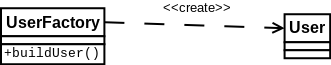
\includegraphics[scale=0.5]{images/27.png}}
\cornell{Aggregazione}{Relazione "Parte Di"\\
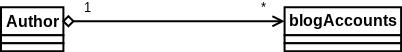
\includegraphics[scale=0.5]{images/28.png}\\
Author è un "aggregato di blogAccounts", non può esistere un Author senza almeno un blogAccount.\\
Le aggregazioni possono essere condivise.}
\cornell{Composizione}{ 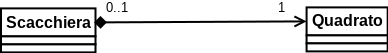
\includegraphics[scale=0.5]{images/29.png}\\
Come l'aggregazione, ma: \begin{itemize}
\item Le parti appartengono ad \textbf{un solo aggregato}
\item \textbf{Solo l'oggetto intero} (scacchiera) \textbf{può creare e distruggere} le sue parti (Quadrato)
\end{itemize}}
\cornell{Classi di Associazione}{Aggiungono attributi e operazioni alle associazioni.\\
Esiste \textbf{solo un'istanza} della classe associazione fra le due classi.\\
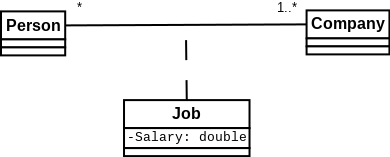
\includegraphics[scale=0.5]{images/30.png}\\
Una persona ha \textbf{un solo} lavoro in un'azienda\\
Questa dicitura mostra dei vincoli che non sarebbero visibili dal codice.\\
Se volessi modellare più lavori per ciascuna azienda, dovrei usare:\\
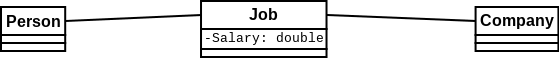
\includegraphics[scale=0.5]{images/31.png}}
\cornell{Generalizzazione}{A generalizza B se ogni oggetto di B è anche un oggetto di A. Quindi abbiamo a che fare con una relazione IS-A.\\
Equivale all'ereditarietà dei linguaggi di programmazione.\\
L'ereditarietà multipla è possibile, ma \textbf{va evitata}\\
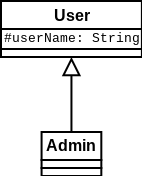
\includegraphics[scale=0.5]{images/32.png}\\
La classe derivata eredita dalla classe base, quindi i campi/operazioni ereditati non vanno inseriti nella classe derivata (a meno di override.)}
